\documentclass[10pt, conference, a4paper, final]{IEEEtran}
\IEEEoverridecommandlockouts
\usepackage{amsmath, amssymb}
\usepackage{fontawesome5}

\usepackage{amsmath}
\usepackage{amssymb}
\usepackage[margin=1in]{geometry} % Adjust margins if needed
\usepackage{graphicx} % Required for including images
\usepackage{subcaption}
\usepackage{algorithm, algorithmicx} % For algorithms
\usepackage[table,xcdraw]{xcolor} % For colored tables
\usepackage{paralist}
%\usepackage{enumitem} % For better control over list
\usepackage{microtype} % Improves typography
\usepackage{tikz}
\usetikzlibrary{fit}
\usepackage{marginnote}
\usepackage{xspace}

% Combine graphicx package loading
\usepackage{float}
\usepackage{booktabs} % For professional looking tables


\makeatletter
\if@twocolumn
  \setlength{\marginparwidth}{20mm}
  \newcommand{\nb}[1]
  {%
   \begingroup%
   \ifodd\value{page}
     \if@firstcolumn\reversemarginpar\fi
   \else
     \if@firstcolumn\else\reversemarginpar\fi
   \fi
   \textcolor{red}{\bf!!}%{\color{red}\it\par[[#1]]\par}
   \marginnote[%\parbox{\marginparwidth}
{\scriptsize\textcolor{red}{#1}}]%
   {%\parbox{\marginparwidth}
{\scriptsize\textcolor{red}{#1}}}%
   \endgroup%
  }
\else
  \setlength{\marginparwidth}{40mm}
  \newcommand{\nb}[1]{\textcolor{red}{\bf!}%
    \reversemarginpar
    \marginpar[\parbox{\marginparwidth}{\scriptsize\textcolor{red}{\raggedleft #1}}]%
    {\parbox{\marginparwidth}{\scriptsize\textcolor{red}{\raggedright #1}}}}
\fi
\makeatother


\newtheorem{example}{Example}



\renewcommand{\S}{\mathcal{S}}
\newcommand{\D}{\mathcal{D}}
\newcommand{\F}{\mathcal{F}}

\newcommand{\adv}{\textsc{adv}}
\newcommand{\noise}{\textsc{noi}}
\newcommand{\translation}{\textsc{tra}}
\newcommand{\scale}{\textsc{sca}}
\newcommand{\shear}{\textsc{she}}
\newcommand{\rotation}{\textsc{rot}}
\newcommand{\contrast}{\textsc{con}}
\newcommand{\brightness}{\textsc{bri}}
\newcommand{\blur}{\textsc{blu}}
\newcommand{\occlusion}{\textsc{occ}}


\newcommand{\gaussian}{\textsc{gau}\xspace}
\newcommand{\saltpepper}{\textsc{sap}}

\newcommand{\testifai}{\textsc{TestifAI}\xspace}
\newcommand{\avec}[1]{\boldsymbol{#1}}



\title{TestifAI: A Comprehensive Testing Framework for Safe AI}
\author{Author Name}
\date{\today}

\begin{document}

\maketitle

\begin{abstract}

    Deep learning (DL) models are critical in high-stakes domains such as autonomous driving, medical diagnostics, and security systems, where their deployment in real-world scenarios requires rigorous robustness testing due to diverse environmental conditions. Traditional metrics like neuron coverage, while essential, do not fully capture all corner cases, which can lead to unexpected model failures. To address this gap, this research introduces a comprehensive testing framework that enhances the correctness evaluation of models through a structured five-stage process. The first stage is specification, defines essential system properties to guide the entire testing process and ensure comprehensive coverage. The second sampling stage, gathering relevant samples for exhaustive model testing. In the test case generation stage, the defined properties are applied to create targeted test scenarios. The testing and probabilistic graph stage validates the effectiveness of these test cases and conducts robustness assessments both locally (within individual category) and globally (across multiple scenarios), employing a Bayesian network for detailed probabilistic and quantitative analysis of performance. The final stage is error summarisation, compiles and analyzes recorded errors to generate actionable graphical error reports and recommendations, thus guiding the refinement of models. This framework not only fills existing gaps in DL testing but also supports the development of models that are correct across varied environmental conditions.
\end{abstract}


\section{Introduction}

% General Problem

% What has been done / citations

% Your more specific problem

% What has been done / what hasn't been done

% Stating your exact problem/objective for the paper

% List the contributions

% Structure of the paper (optional)


Deep neural networks (DNNs) are being more widely used in a variety of applications, yet their correctness in practical applications remains a challenge.

Unlike traditional software, DNNs do not have a clear control-flow structure. They learn their decision policy through training on a large dataset, adjusting parameters gradually using several methods to achieve desired accuracy. Consequently, traditional software testing methods like functional coverage, branch coverage, etc. cannot be applied to DNNs, thereby challenging their use for safety-critical applications. Traditional software testing methods fail when applied to DNNs because the code for DNNs holds no information about the internal decision-making logic.

\begin{itemize}
\item Input space is extremely large, \textbf{unguided simulation} are highly unlikely to find erroneous behaviour
\item Standards available in industry but \textbf{lack of logcial structure} and \textbf{system specification}  
\item Heavily depend on manual collections of test data under different conditions which become expensive as number of test condition increases
\item  Existing coverage criteria are not detailed enough to notice precise behaviours exhibited by DL systems.
\end{itemize}

% \section{Research Goal}
% This paper aims to develop a systematic framework for evaluating local (in a specific region of the input space) and global (across a broad range of inputs) correctness in deep learning models. 
% The goal is to provide a comprehensive error summary to improve model design and training, ensuring their reliability for real-world applications.

By systematically addressing each aspect from initial specifications to detailed error analysis, we aim to enhance the model's accuracy and reliability in real-world scenarios.


This research makes the following key contributions to the field of deep learning correctness evaluation:
\begin{itemize}
   
    \item We design an \textbf{end-to-end pipeline} for evaluating the correctness of system.
    
    \item We propose a \textbf{conceptual framework} that quantifies both local  and global correctness,with formalized Bayesian probabilistic approach to verify system robustness.
    \item A novel \textbf{error summarization}  approach which allows better identification of model weaknesses related to class and property.

    \item We perform all our \textbf{experiments} using publicly available deep learning models and MNIST dataset.
\end{itemize}



\section{Background and Related Research}

\subsection{Deep Neural Networks and AI Systems}

Deep neural networks (DNNs) mimic human brain structure, consisting of  millions of interconnected neurons. They extract high level features from raw input using labeled training data without any human interference.

Formally, a DNN is a function $f\colon\mathbb{R}^{s_0}\mapsto \mathbb{R}^{s_k}$ that takes as input a vector of size $s_0$ and produces a vector of size $s_k$. The function $f$ is computed by composing $k$ layers $L_1\colon\mathbb{R}^{s_0} \mapsto\mathbb{R}^{s_1}, \dots, L_k\colon\mathbb{R}^{s_{k-1}}\mapsto\mathbb{R}^{s_k}$ as $f(x) = L_k(\cdots L_2(L_1(x))\cdots)$.
%
Each layer~$L_i$ typically implements a non-linear function. For instance, a \emph{fully-connected} layer linearly transforms its input $x_{i-1}$ as $W x_{i-1} + b$, where $W\in\mathbb{R}^{s_{i} \times s_{i-1}}$ is the matrix of weights and $b\in\mathbb{R}^{s_i}$ is the bias vector, and then applies to it a non-linear activaion funciton (e.g., sigmoid or Rectified Linear Unit (ReLU)) component wise, generating the output vector $x_i$. For such a layer, the weights specify how its input neurons are connected to its output neurons and are known as \emph{DNN parameters}. For more information about DNNs, we refer the reader to \cite{dnn_archi,Hassija, Liang}.
%
The objective of DNNs training is to learn parameters during training in order to make accurate prediction on unseen data during real world deployment.
%
When the prediction task is that of classification, then $s_k$ represents the number of classes. Assuming that $f(x) = (y_1,\dots,y_{s_k})$, the \emph{classification result} is $\displaystyle\mathop{\text{argmax}}_{i=1}^{s_k} y_i$, which is the index of the component with the highest probability $y_i$. By abuse of notation, sometimes we write $f(x)=c$ to denote the fact that $x$ was classified as $c$. We also write $f(x)_c$ to refer to $y_c$ which represents the probability of $x$ being in class $c$.



By an \emph{AI system} we refer to any software system that is capable to perform complex tasks through use of data, algorithms and high computational power, that typically require human intelligence. These tasks include problem solving, reasoning, decision making and natural language understanding.
%
Deep learning is a subset of AI, that utilise  deep neural networks (DNNs) for complex patterns recognition. Some AI systems are solely based on DNN components. In contrast, \emph{hybrid} AI systems combine DNNs with traditional software to produce the final output.

\begin{figure}{}
    \centering
    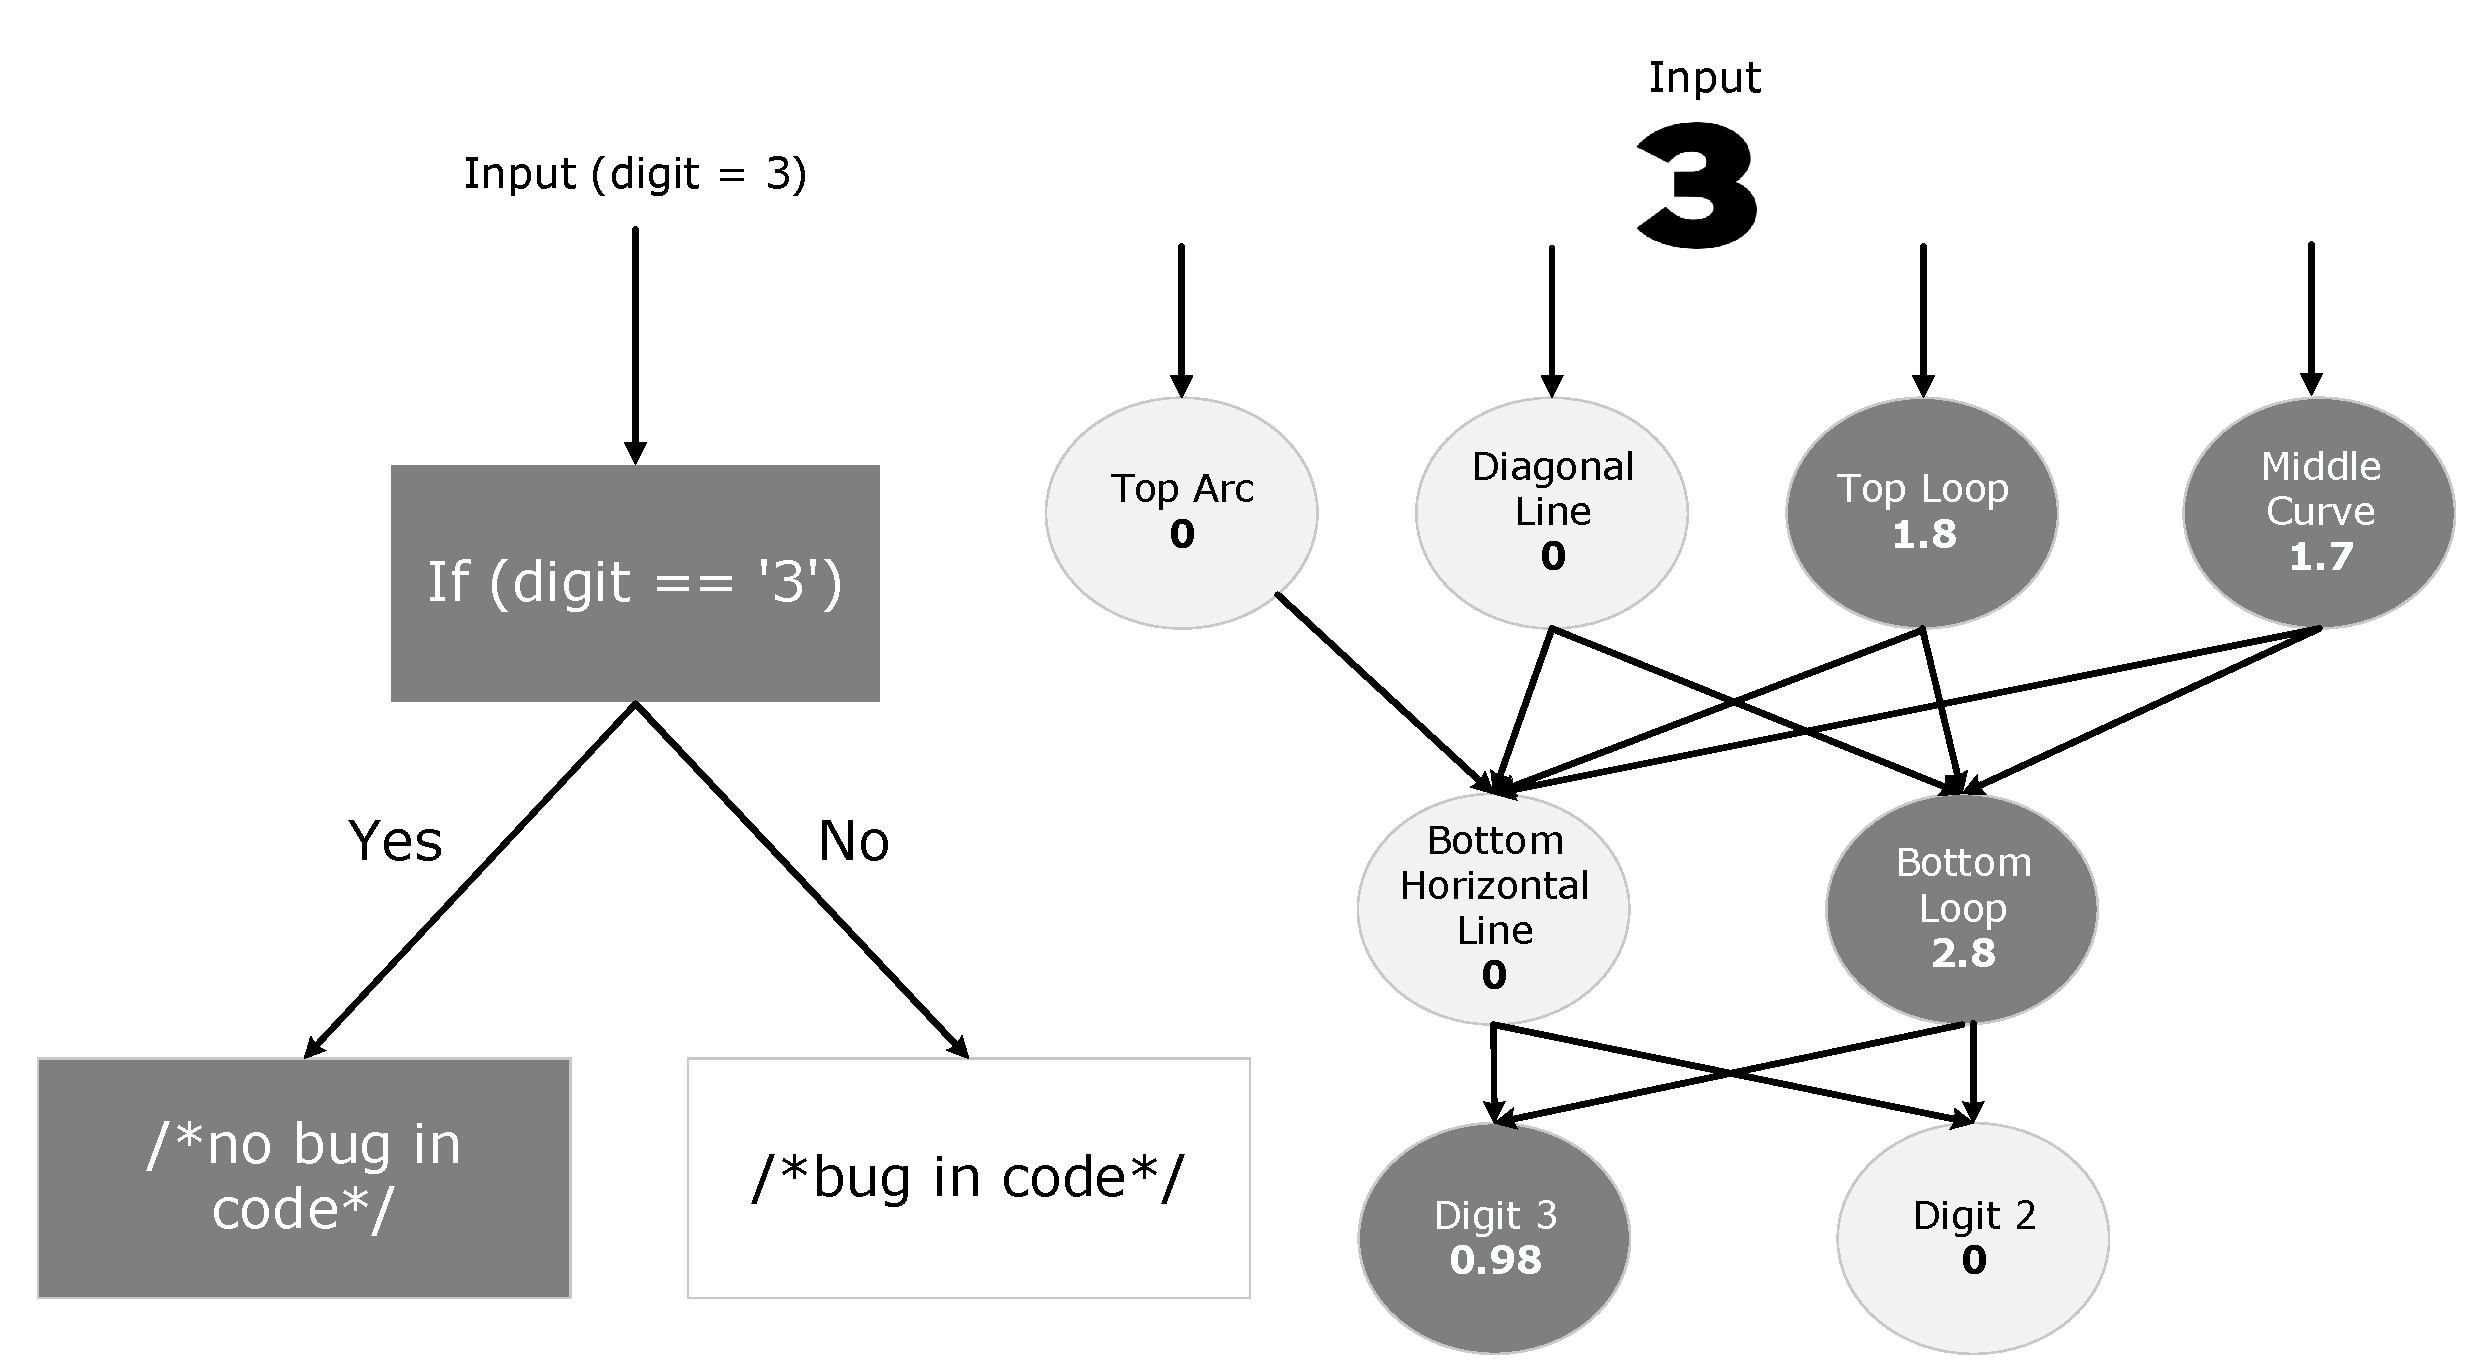
\includegraphics[width=\linewidth]{paper_images/traditional and DNN.pdf}
    \caption{ Comparison between program flows of a traditional program (left) and a neural network (right). The nodes in gray denote the corresponding basic blocks or neurons that participated while processing an input.}
    \label{fig:graph}
\end{figure}


\subsection{Robustness of DNNs}% Realistic Image Perturbations}

% DNNs are known to be not robust. In research, DNNs have been shown to be vulnerable to two main categories of adversaries: \emph{adversarial attacks} \cite{adv_attacks} and \emph{input transformations} \cite{deeptest}.

% \emph{Adversarial attacks} involve carefully crafted perturbations that subtly alter input data to mislead the model into making incorrect predictions:
% \begin{itemize}
%     \item \textbf{Fast Gradient Sign Method (FGSM)}: Alters input pixels in the gradient direction, causing misclassifications with minimal change.
%     \item \textbf{Basic Iterative Method (BIM)}: Enhances FGSM by applying multiple iterations for stronger perturbations.
%     \item \textbf{Carlini and Wagner (C\&W) attack}: Uses optimization to create small perturbations that mislead the DNN with high confidence.
%     \item \textbf{DeepFool}: Iteratively adjusts inputs to cross decision boundaries with minimal perturbations.
%     \item \textbf{Jacobian-based Saliency Map Attack (JSMA)}: Targets specific input features to cause targeted misclassifications
% \end{itemize}

% \emph{Input transformations} involve modifying the input images in ways that can reveal the model's sensitivity to variations:
% \begin{itemize}
%     \item \textbf{Noise}: Introduce various types of noise (e.g., Gaussian noise, salt-and-pepper noise).
%     \item \textbf{Translation}: Move the entire image in one or more directions.
%     \item \textbf{Scaling}: Change the size of the image.
%     \item \textbf{Shear}: Alter the shape of objects within the image.
%     \item \textbf{Rotation}: Rotate the image.
%     \item \textbf{Contrast adjustments}: Modify the contrast of the image.
%     \item \textbf{Brightness changes}: Alter the brightness of the image.
%     \item \textbf{Blurring}: Apply a blur effect to the image.
%     \item \textbf{Occlusion}: Partially hide the image.
% \end{itemize}

Deep Neural Networks (DNNs) are known for their lack of robustness. In research, DNNs have been shown to be vulnerable to two main categories of adversaries: \emph{adversarial attacks}~\cite{adv_attacks} and \emph{image transformations}~\cite{deeptest}.

Let $\mathcal{A}$ denote an adversary. Each category can be described formally as follows:

\smallskip\noindent%
\textbf{Adversarial Attacks $\mathcal{A}_{\text{adv}}$}

(\adv) This involves the generation of perturbations $\delta$ such that $x' = x + \delta$ misleads the DNN $f$ into making incorrect predictions, where $x$ is the original input and $x'$ is the perturbed input. Various methods under this category include:
\begin{itemize}[$\bullet$]
    \item \emph{Fast Gradient Sign Method (FGSM)}: For an input~$x$ and its true label $y$, FGSM generates $x' = x + \epsilon \cdot \text{sign}(\nabla_x J(x, y))$, where $J$ is the loss function and $\epsilon$ is a small perturbation factor.
    \item \emph{Basic Iterative Method (BIM)}: This extends FGSM by iteratively applying small perturbations: $x'^{(i+1)} = x'^{(i)} + \alpha \cdot \text{sign}(\nabla_x J(x'^{(i)}, y))$.
    \item \emph{Carlini and Wagner (C\&W) Attack}: Utilizes optimization to find $\delta$ that minimizes the $L_p$-norm while ensuring $f(x + \delta) \neq y$.
    \item \emph{DeepFool}: Iteratively perturbs $x$ by $\delta$ to move it across decision boundaries.
    \item \emph{Jacobian-based Saliency Map Attack (JSMA)}: Manipulates specific features of $x$ to achieve targeted misclassifications.
\end{itemize}

\smallskip\noindent%
\textbf{Image Transformations $\mathcal{A}_{\text{trans}}$}

\begin{figure*}
  \centering
  
  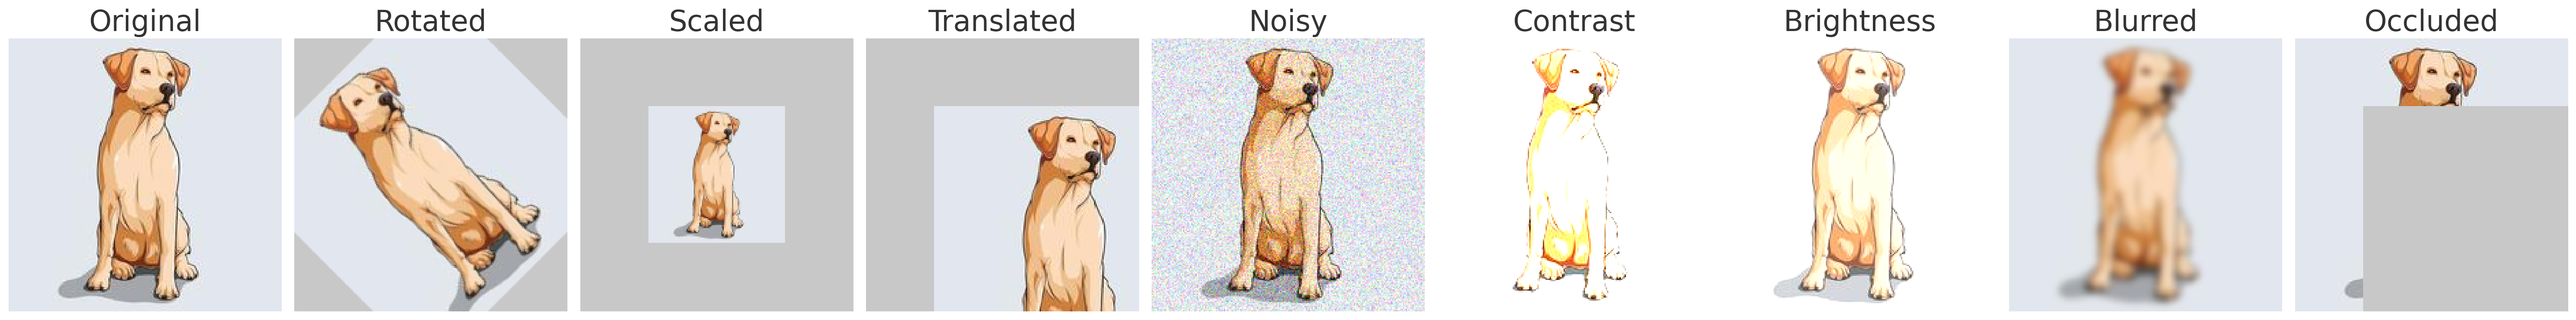
\includegraphics[width=\linewidth]{paper_images/output_update.png}
  
  \caption{Image transformations for ...}
  \label{fig:image-trans}
\end{figure*}

This involve modifying the input images in a manner that exploits the model's sensitivity to variations, potentially causing misclassifications. Various methods under this category include:\nb{Add a figure with examples of these transformations}
\begin{itemize}[$\bullet$]
    \item \emph{Noise Addition}: Introducing noise $\eta$ such that $x' = x + \eta$.  We consider  \emph{Gaussian} noise \gaussian and \emph{salt-and-pepper} noise \saltpepper.
    \item \emph{Translation} (\translation): Shifting the image $x$ by a vector $t$ to obtain $x' = \text{translate}(x, t)$.
    \item \emph{Scaling} (\scale): Resizing the image $x$ by a factor $s$ to get $x' = \text{scale}(x, s)$.
    \item \emph{Shearing} (\shear): Applying a shear transformation to $x$ resulting in $x' = \text{shear}(x, \theta)$.
    \item \emph{Rotation} (\rotation): Rotating the image $x$ by an angle $\theta$ to produce $x' = \text{rotate}(x, \theta)$.
    \item \emph{Contrast Adjustment} (\contrast): Modifying the contrast of $x$, represented as $x' = \text{adjust\_contrast}(x, \alpha)$.
    \item \emph{Brightness Change} (\brightness): Altering the brightness of $x$, yielding $x' = \text{change\_brightness}(x, \beta)$.
    \item \emph{Blurring} (\blur): Applying a blur effect to $x$, giving $x' = \text{blur}(x, k)$, where $k$ is the kernel size.
    \item \emph{Occlusion} (\occlusion): Partially hiding regions of $x$, leading to $x' = \text{occlude}(x, m)$, where $m$ denotes the mask.
\end{itemize}

By analyzing various types of adversaries, our proposed comprehensive testing framework evaluates model robustness, providing probabilities of model effectiveness against each adversary and assessing accuracy under adversarial conditions across different classes within any dataset.


\subsection {DNN Testing Techniques}
The development of DNNs is significantly different from traditional software. The developers explicitly define logic in traditional software but DNNs learn logic rules from the raw data rather than explicitly programmed. The developers shape these rules by modifying the training data, selecting the features and designing the DNNs architecture such as the number of neurons and layers.

Since the logic of a DNN is non-transparent \cite{deepxplore}\nb{E: explain this better, probably need to cite some papers on explainable AI}, we are unable to identify the reasons behind its erroneous behaviour. Therefore, it is crucial to test and correcting its error, particularly in safety-critical systems. Next we briefly introduce two major DNN testing techniques: coverage criteria and test-case generation.

\smallskip\noindent%
\textbf{Coverage Criteria}
In traditional software testing, coverage criteria are used to measure how thoroughly software is tested. In DNNs, coverage might not directly apply to lines of code but rather to the input space or the variety of data the model can effectively handle or provide predictions for.

Neuron coverage (NC) \cite{deepxplore} is the first coverage metric proposed in the literature to test DNNs. It is defined as the ratio of neurons activated by a test input to the total number of neurons in the model, where a neuron is activated when its activation value exceeds a predefined threshold. 

Ma et al. \cite{deepguage}, proposed variety of coverage metrics include: K-multisection neuron coverage (KMNC), Neuron boundary coverage (NBC) and Strong neuron activation coverage (SNAC). KMNC calculates coverage by dividing the interval between lower and upper bounds into k-bins and measuring the number of bins activated by the test inputs. For a test suite, it is the ratio of uniquely covered bins to the total bins in the model. NBC measures the ratio of corner case regions covered by test inputs, with corner cases defined as activation values below or above those observed during training. SNAC similarly measures how many upper corner cases, defined as activation values above the training range, are covered by test inputs. 

Modified Condition/Decision Coverage (MC/DC) \cite{SunY} coverage metric  capture causal changes in test inputs based on the sign and value change of a neuron's activation. 

Likelihood-based Surprise Adequacy (LSA) uses Kernel Density Estimation (KDE) to estimate the likelihood of a test input during the training phase, prioritizing inputs with higher LSA scores as they are closer to classification boundaries. Distance-based Surprise Adequacy (DSA) is an alternative to LSA that uses the distance between activation traces of new test inputs and those observed during training \cite{KimJ}.\nb{E: add references}

\smallskip\noindent%
\textbf{DNN Test-case Generation}



Test-case generation methods are influenced by traditional software testing methods like fuzz testing, metamorphic testing and symbolic execution. In the following sections, we will explore the current state of art research in DNN test generation.

DeepXplore \cite{deepxplore} is a whitebox test-case generation method that checks how different DNNs behave using domain specific rules on inputs. It uses multiple models trained on same data to find differences in their prediction. It aims to jointly optimize neuron coverage and different prediciton  between models, using gradient ascent for test generation.


DeepTest \cite{deeptest} is another testing technique focuses on generating test inputs for autonomous cars by applying domain specific rules on seed inputs. It uses a greedy search method based on NC metric to create effective test cases.

Adapting traditional fuzzing technique for DNNs test-case generation method with techniques like DLFuzz \cite{dlfuzz} and TensorFuzz \cite{tensorfuzz}. DLFuzz genrates adversarial inputs based on NC, akin to DeepXplore \cite{deepxplore}, but does not require multiple models and use constraints to keep new inputs similar to originals. TensorFuzz, on the other hand, employs covergae-guided testing to uncover numerical issues and discrepancies in DNNs and their quantized verisons.

DeepConcolic \cite{deepconcolic} employs a concolic testing approach to generate adversarial inputs for DNN testing. It combines symbolic execution with concrete execution path information to meet coverage criteria, supporting both NC and MC/DC criteria.


Traditional techniques are simple, failing to capture the full complexity and preciseness of model behaviors. Trying to explore all possible behaviors of a model is nearly impossible because there are just too many paths to consider. These metrics also often overlook the detailed interactions that happen within and between layers of the model. When it comes to defining and testing all the necessary decision boundaries, especially in complex models, it becomes a alarming task.  Many of the existing metrics do not provide clear directions for improving the model, leaving you without actionable insights. Scalability and adaptability are other major issues. Many criteria are not scalable or adaptable across diverse model architectures.

In this paper, we address these issues and design a systematic testing framework for .....

\subsection{Bayesian Networks}


Bayesian networks are a powerful probabilistic graphical model that represent a set of variables and their conditional dependencies via a directed acyclic graph (DAG). They are particularly useful for modeling uncertainty in complex systems. The fundamental equation of Bayesian networks is the Bayes theorem, which is given by:

\begin{equation}
P(A|B) = \frac{P(B|A)P(A)}{P(B)}
\end{equation}

This equation allows us to update the probability estimate for a hypothesis as more evidence or information becomes available.

In the context of DNNs, Bayesian networks can offer significant advantages. Behavioral assessment considers probabilistic relationships to offer a richer, more detailed understanding of how different inputs affect model outputs. By developing a strategic focus on high-risk areas, it prioritizes regions with the highest uncertainty or risk for targeted testing, making the process more efficient and effective. 



\section{Approach}
\begin{figure*}{}
    \centering
    % 
\includegraphics[width=\linewidth]{paper_images/frame.pdf}

    \begin{tikzpicture}[component/.style={fill=gray!80, text=white,
        rounded corners, outer sep=1mm, text width=2.6cm, align=flush
        center, minimum height=1.2cm, scale=0.8},
      input/.style={draw, scale=0.8,  inner sep=2mm, outer sep=1mm}]\sf
      
      \foreach \x/\al/\lab in {%
        1/sampl/Sampling,%
        2/gener/Testcase Generation,%
        3/testing/Validation,%
        4/summary/{Error\\ Summarisation}%
      }{ \node[component] (\al) at (3.5*\x,0) {\textbf{\lab}}; }

      \node[fit=(sampl)(summary), draw=gray, ultra thick] (approach) {};

      \node[input] (aisystem) at (0.2, 0.5) {AI System $\S$};
      \node[input] (spec)     at (0.2, -0.5) {Specifications $\Sigma$};

      \foreach/\from/\to in {%
        sampl/gener, gener/testing, testing/summary%
      }{ \draw[-stealth, very thick] (\from) -- (\to); }

      \draw[-latex, thick] (aisystem) -- (approach.179);
      \draw[-latex, thick] (spec) -- (approach.181);
    \end{tikzpicture}
    \caption{Overview of the \testifai Framework}
    \label{fig:framework}
\end{figure*}

This section introduces our comprehensive approach to evaluating an AI system performance, summarised in Figure~\ref{fig:framework}. It takes as input the description of an AI system and a set of relevant specifications against which the AI system should be checked. The framework itself has 4 main components: % This step-by-step method highlights the strengths and weaknesses of the AI system.
\begin{inparaenum}[\it (i)]
% \item The process begins with a detailed description of the properties that need to be tested.
\item \emph{Sampling} to choose the original inputs for the AI system;
\item \emph{Testcase generation} to generate the specific test cases from the sampled inputs according to the specifications;
\item \emph{Validation} to check the behaviour of the AI system on the generated test-cases, where the check can be fully-fledged \emph{verification} or more light-weight \emph{testing};
  % To thoroughly assess the model, we generate (testcase generation) and test (testing) specific cases based on these properties.  
\item \emph{Error summarisation} to quantify the performance of the AI system in terms of its global/local robustness/correctness.
  % Following this, we summarise the errors, focusing on how individual image performance (local correctness) translates to the overall system performance (global correctness).  
\end{inparaenum}



We focus on AI systems with DNN components performing classification tasks. We assume that an AI system $\S$ is a pair $(\F,\D)$ where
\begin{itemize}[$\bullet$]
\item $\F$ is the functional unit consisting of $n$ DNN \emph{classifiers} $f_1,\dots,f_n$ and a symbolic (software) component~$\omega$ such that given an input $\avec{x}=(x_1,\dots,x_n)$, the \emph{output}~$\F(\avec{x})$ is defined as $\omega(f_1(x_1),\dots,f_n(x_n))$.
  % 
\item $\D$ (for dataset) is a structure that describes valid inputs for each classifier $f_i$ and the corresponding correct outputs (i.e., labels). In particular, $\D.\mathit{next}_i(\mathit{param})$ returns a valid input $x_i$ for $f_i$, given the parameter $\mathit{param}$.\nb{E: elaborate here what param is} Moreover, $\D.N_i$ is the number of distinct class labels for each classifier~$f_i$.
\end{itemize}

\begin{example}
  \label{ex:mnist-adder}
  An instance of a simple AI system is an \emph{MNIST Digit Adder} $\S_{\text{MNIST}} = (\F,\D)$, where $\F = (\{f_{\text{mnist}}\}, +)$, $f_{\text{mnist}}$ is an MNIST Digit classifier and $\F$ takes as input two MNIST Digit images, recognises the digits in the images and computes their sum, i.e., $\F(x_1,x_2) = f_{\text{mnist}}(x_1) + f_{\text{mnist}}(x_2)$. $\D$ is the testing dataset for MNIST Digit consisting of 10,000 labelled images.
\end{example}

\smallskip

We assume that \emph{specifications} $\Sigma$ is a pair $(P, V)$,
where $P$ is a set of perturbations against which we are
characterising the behaviour of $\S$. Each perturbation comes with the
parameters to instantiate the set of all possible perturbations. 
%
Furthermore, $V$ is a validation flag, if $V=t$, then we do testing,
and if $V=v$, we do verification.

\begin{example}
  To evaluate the correctness of the MNIST Digit Adder
  $\S_{\text{MNIST}}$, we define the specifications $\Sigma = (P, V)$
  as follows:
  $P = \{\gaussian(0,0.1), \saltpepper(200:255, 0:5, 0.2),
  \rotation(3,30,3)\}$ and $V=t$. Here, $\gaussian(0,0.1)$ specifies
  Gaussian noise with the mean of $0$ and standard deviation of $0.1$,
  $\saltpepper(200:255,0:5,0.2)$ specifies salt and pepper noise,
  where 10\% of pixels are `bleached' up to the values 200 to 255 and
  10\% of pixels are darkened to the values between 0 and 5, and
  $\rotation(3,30,3)$
  specifies the set of rotations with the minimum rotation angle of 3,
  maximum of 30 and the step size of 3.
  % Specifically, we apply the following perturbations to the input
  % images $x_1$ and $x_2$:
  % \begin{itemize} 
  % \item \textbf{Rotation}: Each input image will be rotated by a
  %   specified angle, $\theta$. Let $x_1' = \text{rotate}(x_1, \theta)$
  %   and $x_2' = \text{rotate}(x_2, \theta)$. We then compute:
  %
  %   $\F(x_1', x_2') = f_{\text{mnist}}(x_1') + f_{\text{mnist}}(x_2')$
  % \item \textbf{Noise}: Gaussian noise with mean $\mu$ and standard
  %   deviation $\sigma$ will be added to each input image. Let
  %   $x_1'' = \text{noise}(x_1, \mu, \sigma)$ and
  %   $x_2'' = \text{noise}(x_2, \mu, \sigma)$. We then compute:
  %
  %   $\F(x_1'', x_2'') = f_{\text{mnist}}(x_1'') + f_{\text{mnist}}(x_2'')$
  %   \end{itemize}
\end{example}

\smallskip

In what follows, we assume fixed the inputs, an AI system $\S=(\F,\D)$
and specifications $\Sigma=(P,V)$.

\subsection{Sampling}
The sampling process involves a random but balanced choice of samples from each class, focusing exclusively on instances that the model has correctly predicted.
%
Sampling happens independently for each classifier $f_i$. To ensure a representative and fair distribution of data across all classes, we sample the same number of instances from each class. The full sample $S_i$ for classifier $f_i$, $i=1,\dots,n$, is computed as:

\begin{equation}
S_i = \bigcup_{c=1}^{\D.N_i} S_i^c
\end{equation}
%
where $S_i^c$ is a subset of the correctly classified samples for a class $c$ consisting of $M_i$ (the number of samples for each class specific to $f_i$) elements:
\[S_i^c = \big\{x = \D.next_i(class=c)\mid f_i(x)=c\big\}|_{M_i}\] Note that each sample is obtained by a call to the method $\D.next_i$.

\begin{example} Recall the MNIST Digit Adder system $\S_{\text{MNIST}}$ from Example~\ref{ex:mnist-adder}.
  %
  When sampling, we make sure to select only correctly classified
  samples. For each digit $c$ (0 to 9), we randomly sample 100 images,
  i.e., $samp_1(\D,c,100)$ contains 100 inputs $x$ such that
  $f_{\text{mnist}}(x) = c$. In total, $S_1$ contains 1000 samples for
  all 10 classes.
\end{example}

  \subsection{Test Case Generation}
  The test case generation process aims to create test cases based on the given specifications to evaluate the correctness/robustness of the AI system.

  Let $S_i^c$ be the set of samples produced in the sampling step for the classifier $f_i$ and a class $c$. For each perturbation $p\in P$, we generate a set $\T_p^c$ of test cases. Specifically, for each sample $x\in S$ we produce $testcases(p,c,x)$ according to $p$. Then $\T_p^c = \bigcup_{x\in S} testcases(p,c,x)$.
  
  \begin{example}
    To generate test cases for the MNIST Digit Adder $\S_{\text{MNIST}}$, we use the specifications defined in Example 2, which include noise and rotation perturbations. Let $S$ be the set of sampled images obtained in Example 3. For each pair of images $(x_1, x_2) \in S$, we define the following test cases:
    \begin{itemize}
        \item \textbf{Rotation}: For a given angle $\theta$, generate the perturbed images $x_1' = \text{rotate}(x_1, \theta)$ and $x_2' = \text{rotate}(x_2, \theta)$. The test case is then:
        $\mathcal{T}_{\text{rotation}} = \left\{(x_1', x_2') \mid x_1', x_2' \in \text{rotate}(S, \theta)\right\}$
        \item \textbf{Noise}: For a given mean $\mu$ and standard deviation $\sigma$, generate the perturbed images $x_1'' = \text{noise}(x_1, \mu, \sigma)$ and $x_2'' = \text{noise}(x_2, \mu, \sigma)$. The test case is then:
        $\mathcal{T}_{\text{noise}} = \left\{(x_1'', x_2'') \mid x_1'', x_2'' \in \text{noise}(S, \mu, \sigma)\right\}$
    \end{itemize}
    The overall set of test cases $\mathcal{T}$ is the union of the individual test cases:
    $\mathcal{T} = \mathcal{T}_{\text{rotation}} \cup \mathcal{T}_{\text{noise}}$
   
\end{example}
% This section outlines the generation of test cases to assess model robustness through properties such as noise, rotation, brightness adjustments, occlusion, and scaling.

% \begin{itemize}
%     \item \textbf{Noise Addition:} Noise is added to an image $x_i$ using a Gaussian noise model. The noise function $p_n$ is defined as:
%     \[ p_n(x_i, \sigma) = x_i + \epsilon \]
%     where $\epsilon \sim \mathcal{N}(0, \sigma)$ denotes the Gaussian noise with mean zero and standard deviation $\sigma\).

%     \item \textbf{Rotation:} The rotation of an image $x_i$ by an angle $\theta\) is modeled by the rotation function $p_r$:
%     \[ p_r(x_i, \theta) = \text{rotate}(x_i, \theta) \]
%     where $\text{rotate}(\cdot, \theta)\) represents the rotation operation.

%     \item \textbf{Brightness Adjustment:} Brightness adjustment of an image $x_i$ is controlled by a multiplicative factor $\beta$, which scales the intensity of all pixels. The brightness function $p_b$ can be defined as:
%     \[ p_b(x_i, \beta) = \beta \cdot x_i \]
%     where $\beta > 1$ increases brightness, and $\beta < 1$ decreases it. This approach ensures that the image's contrast is preserved while adjusting its brightness.

%     \item \textbf{Occlusion:} Occlusion is simulated by covering parts of the image $x_i$ with a mask $M$. The occlusion function $p_o$ is defined as:
%     \[ p_o(x_i, M) = x_i \cdot M \]
%     where $M$ is a binary mask that obscures parts of the image, with $M = 0$ for occluded pixels and $M = 1$ for visible pixels.

%     \item \textbf{Scaling:} Scaling of an image $x_i$ is controlled by a scaling factor $s$, which resizes the image. The scaling function $p_s$ is defined as:
%     \[ p_s(x_i, s) = \text{scale}(x_i, s) \]
%     where $\text{scale}(\cdot, s)\) represents the scaling operation, resizing the image by a factor of $s$.
% \end{itemize}


\subsection{Validation}

In this step we run the validation queries for each test case generate previously.
% The Testing section evaluates how accurately and confidently the  AI subsystem's predicts under various properties applied to images from each class. This phase focuses on directly measuring and quantifying the correctness of the  AI subsystem's.

Let $f_i$ be a classifier, $x$ an input and $c$ the correct class label of $x$.  Denote by $query(f_i,x,c)$ the outcome of the validation query defined as $1$ if $f_i(x)=c$ and as $0$ otherwise. 

Fix $p\in P$ and a class $c$. For every test case in $\T_p^c$, we store the results in the form \[Raw_{p,c} = \Big\{\big(query(f_i,x,c),\ f_i(x)_c\big) \mid x \in \T_p^c\Big\}\]  



After generating test cases, measure the  AI subsystem's confidence for each class under each type of property.


    \subsubsection{Local Correctness}

    Local correctness involves checking the AI subsystem's performance on individual images subjected to different transformations. For each image $x$ from a set of samples $X$, the AI subsystem produces a confidence score $f(x)$ representing its certainty in recognizing the digit. The local correctness for a transformation $T$ applied to an image $x$ is defined as:


    $ \text{Local Correctness}(x, T) = f(T(x))$


    Where $T$ can be any transformation such as noise addition, rotation, brightness adjustment, occlusion, or scaling. Each transformation is evaluated to determine its impact on the confidence score.

    
    \subsubsection{Global Correctness}

    Global correctness evaluates the AI subsystem's performance on combinations of images and transformations, such as adding two digits under different transformations. Given a set of 100 samples for each digit (0-9), we randomly select images to form digit pairs. The global correctness assesses the combined confidence for recognizing the result of operations like addition under each transformation.

    For each transformation $T$, we define local correctness for digits $d_1$ and $d_2$ as follows:
    
    $ \text{LC}_{T}(d_1) = \text{Local Correctness}(x_1, T)$
    $\text{LC}_{T}(d_2) = \text{Local Correctness}(x_2, T)$
    

    Where $x_1$ and $x_2$ are randomly selected images representing digits $d_1$ and $d_2$.
    
    The global correctness for each transformation is then defined as the product of the local correctness values:
    
    $\text{GC}_{T} = \text{LC}_{T}(d_1) \times \text{LC}_{T}(d_2)$
    
    To determine the optimistic and pessimistic global correctness across all transformations, we calculate the following:
    
    \begin{itemize}
        \item \textbf{Optimistic Global Correctness}:

        $\text{GC}_{opt} = \max_{T} (\text{GC}_{T})$
        \item \textbf{Pessimistic Global Correctness}:
    
        $\text{GC}_{pes} = \min_{T} (\text{GC}_{T})$

    \end{itemize}
    
    For the addition operation, if we denote the sum of digits $d_1$ and $d_2$ as $d_{\text{sum}}$, the overall global correctness for the operation is:
    
        $ \text{Overall Global Correctness} = \min(\text{GC}_{opt}, \text{GC}_{pes})$

    
    Where each transformation is evaluated separately, and the global correctness is determined based on the individual probabilities of correct recognition for each digit under each transformation.
    \begin{figure}{}
        \centering
        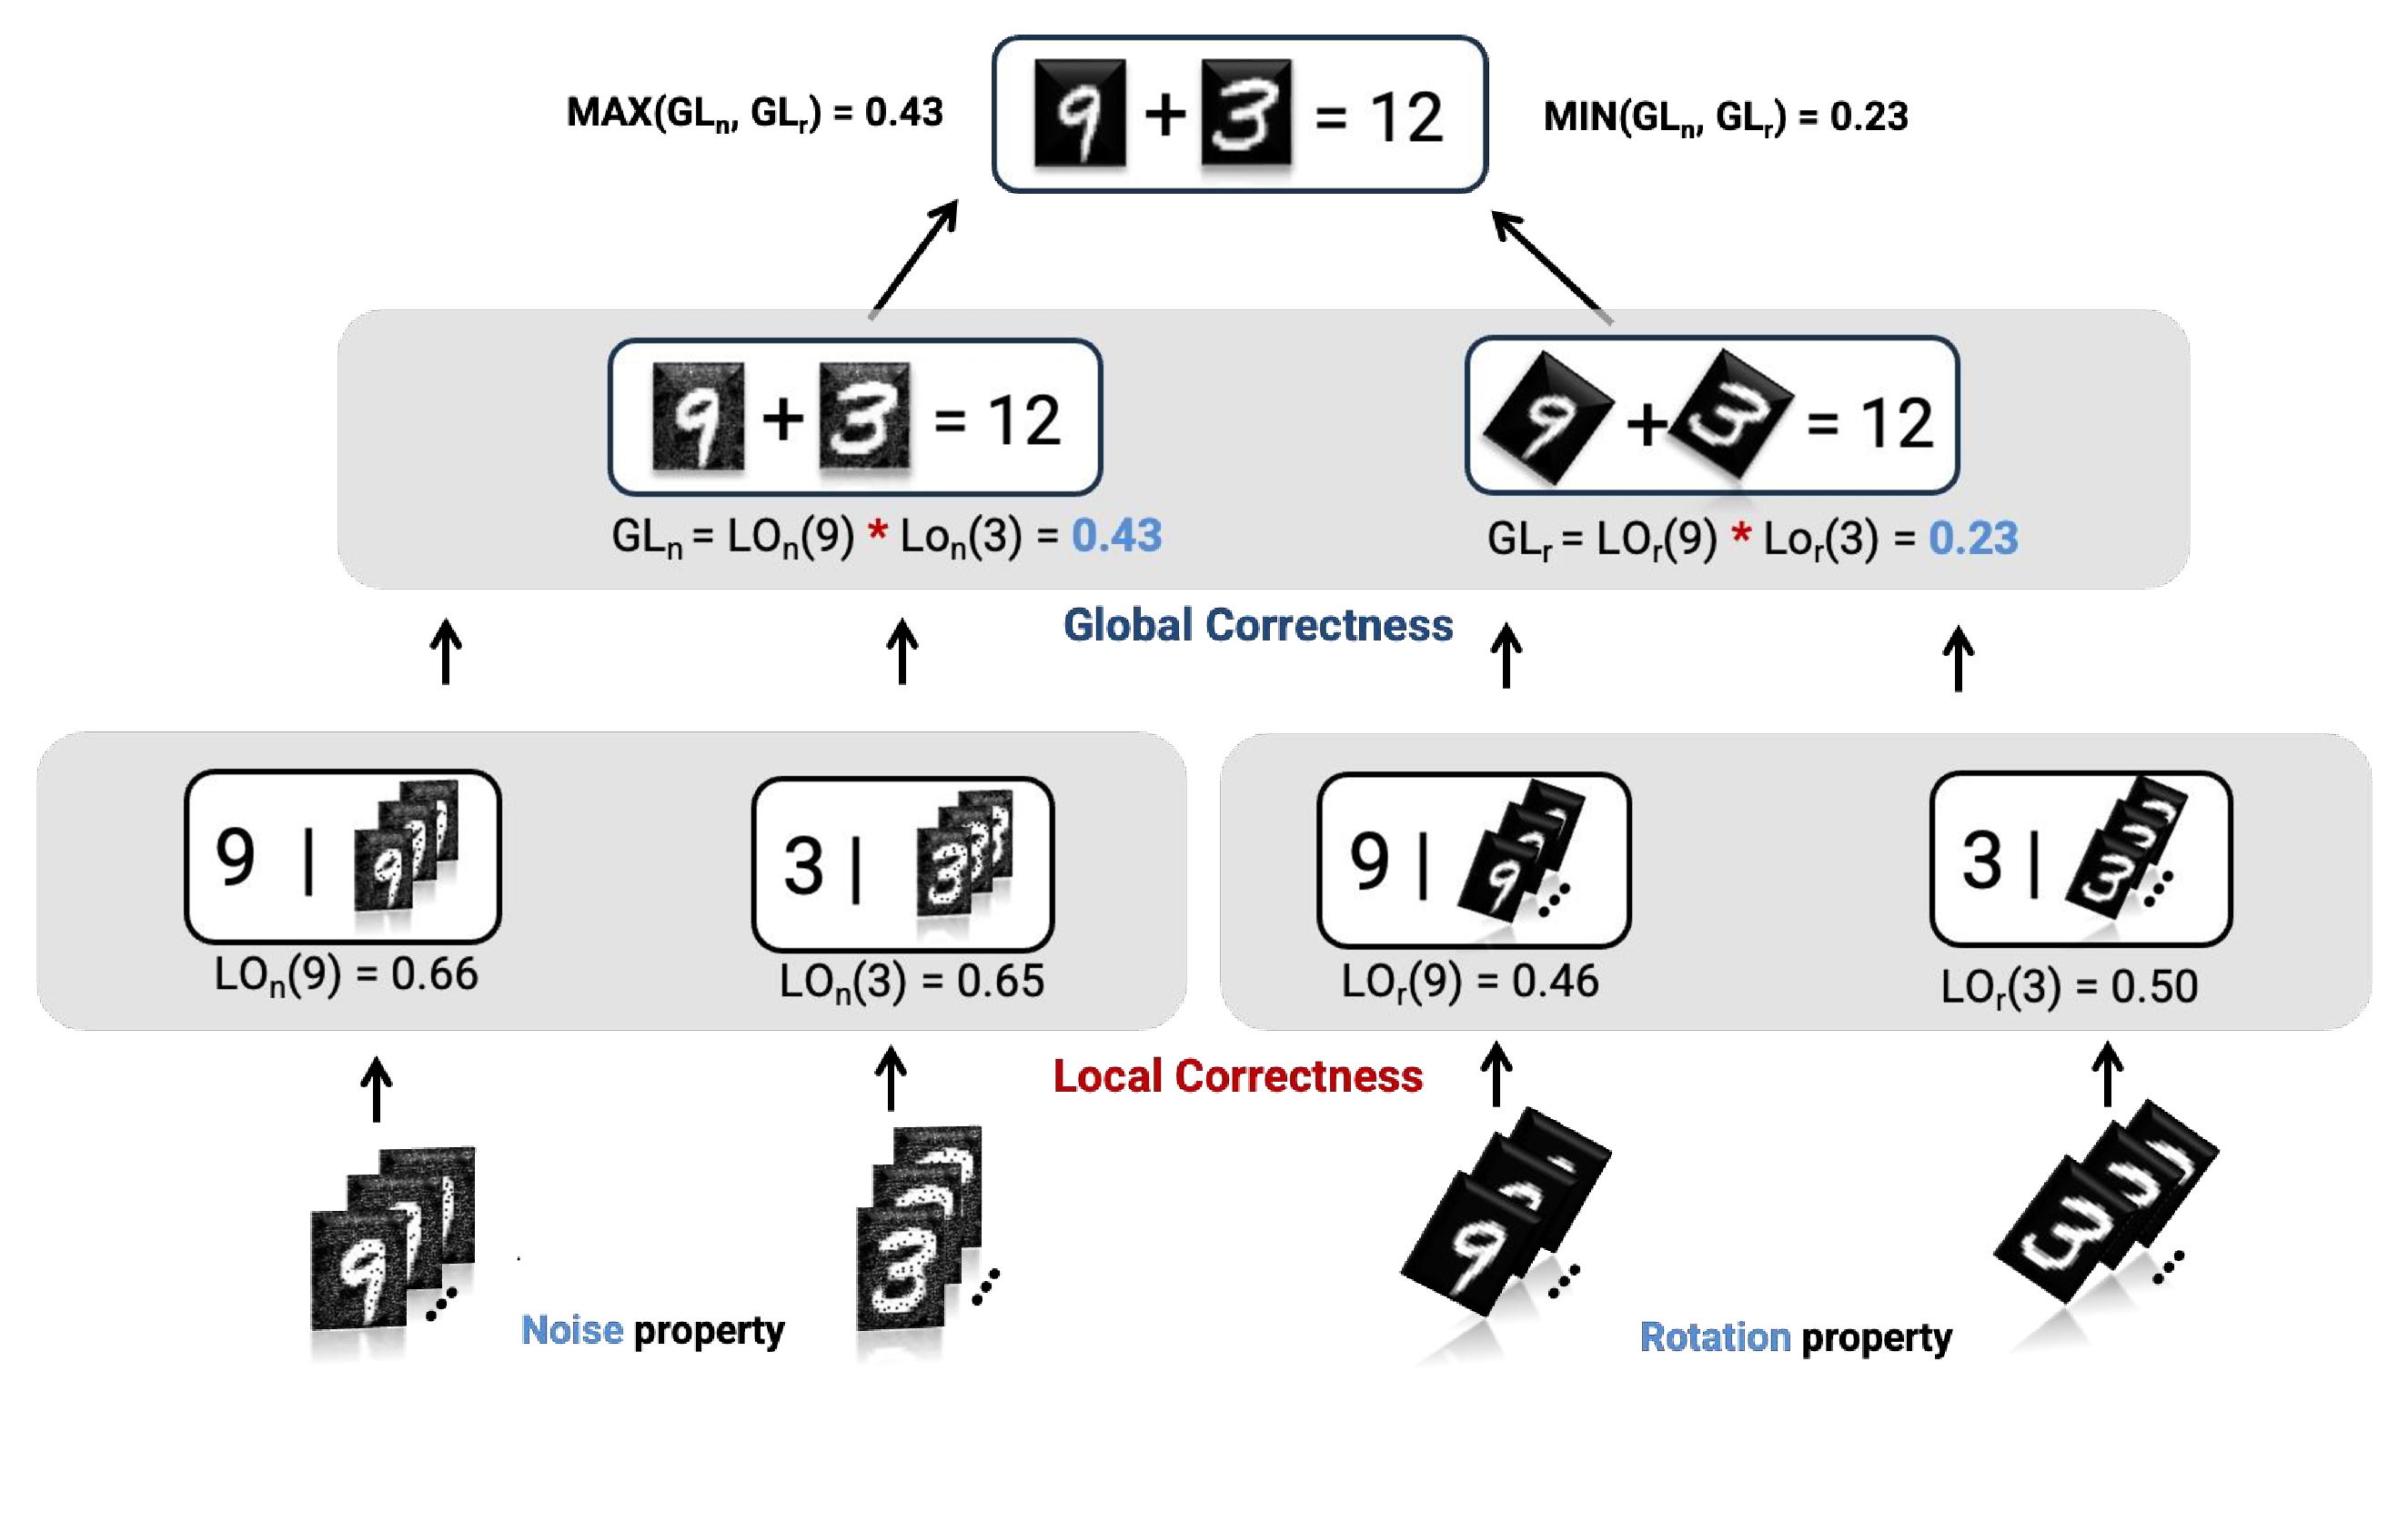
\includegraphics[width=\linewidth]{paper_images/noise_rotation_localcal_global.pdf}
        \caption{Graphical View of Local and Global Correctness}
        \label{fig:graph}
    \end{figure}

 
\subsubsection{how to write bayesian story, either it would be proper section or adust each baesian equation in all steps??? }
\subsection{Error Summarization}

\begin{figure}[H]
    \centering
    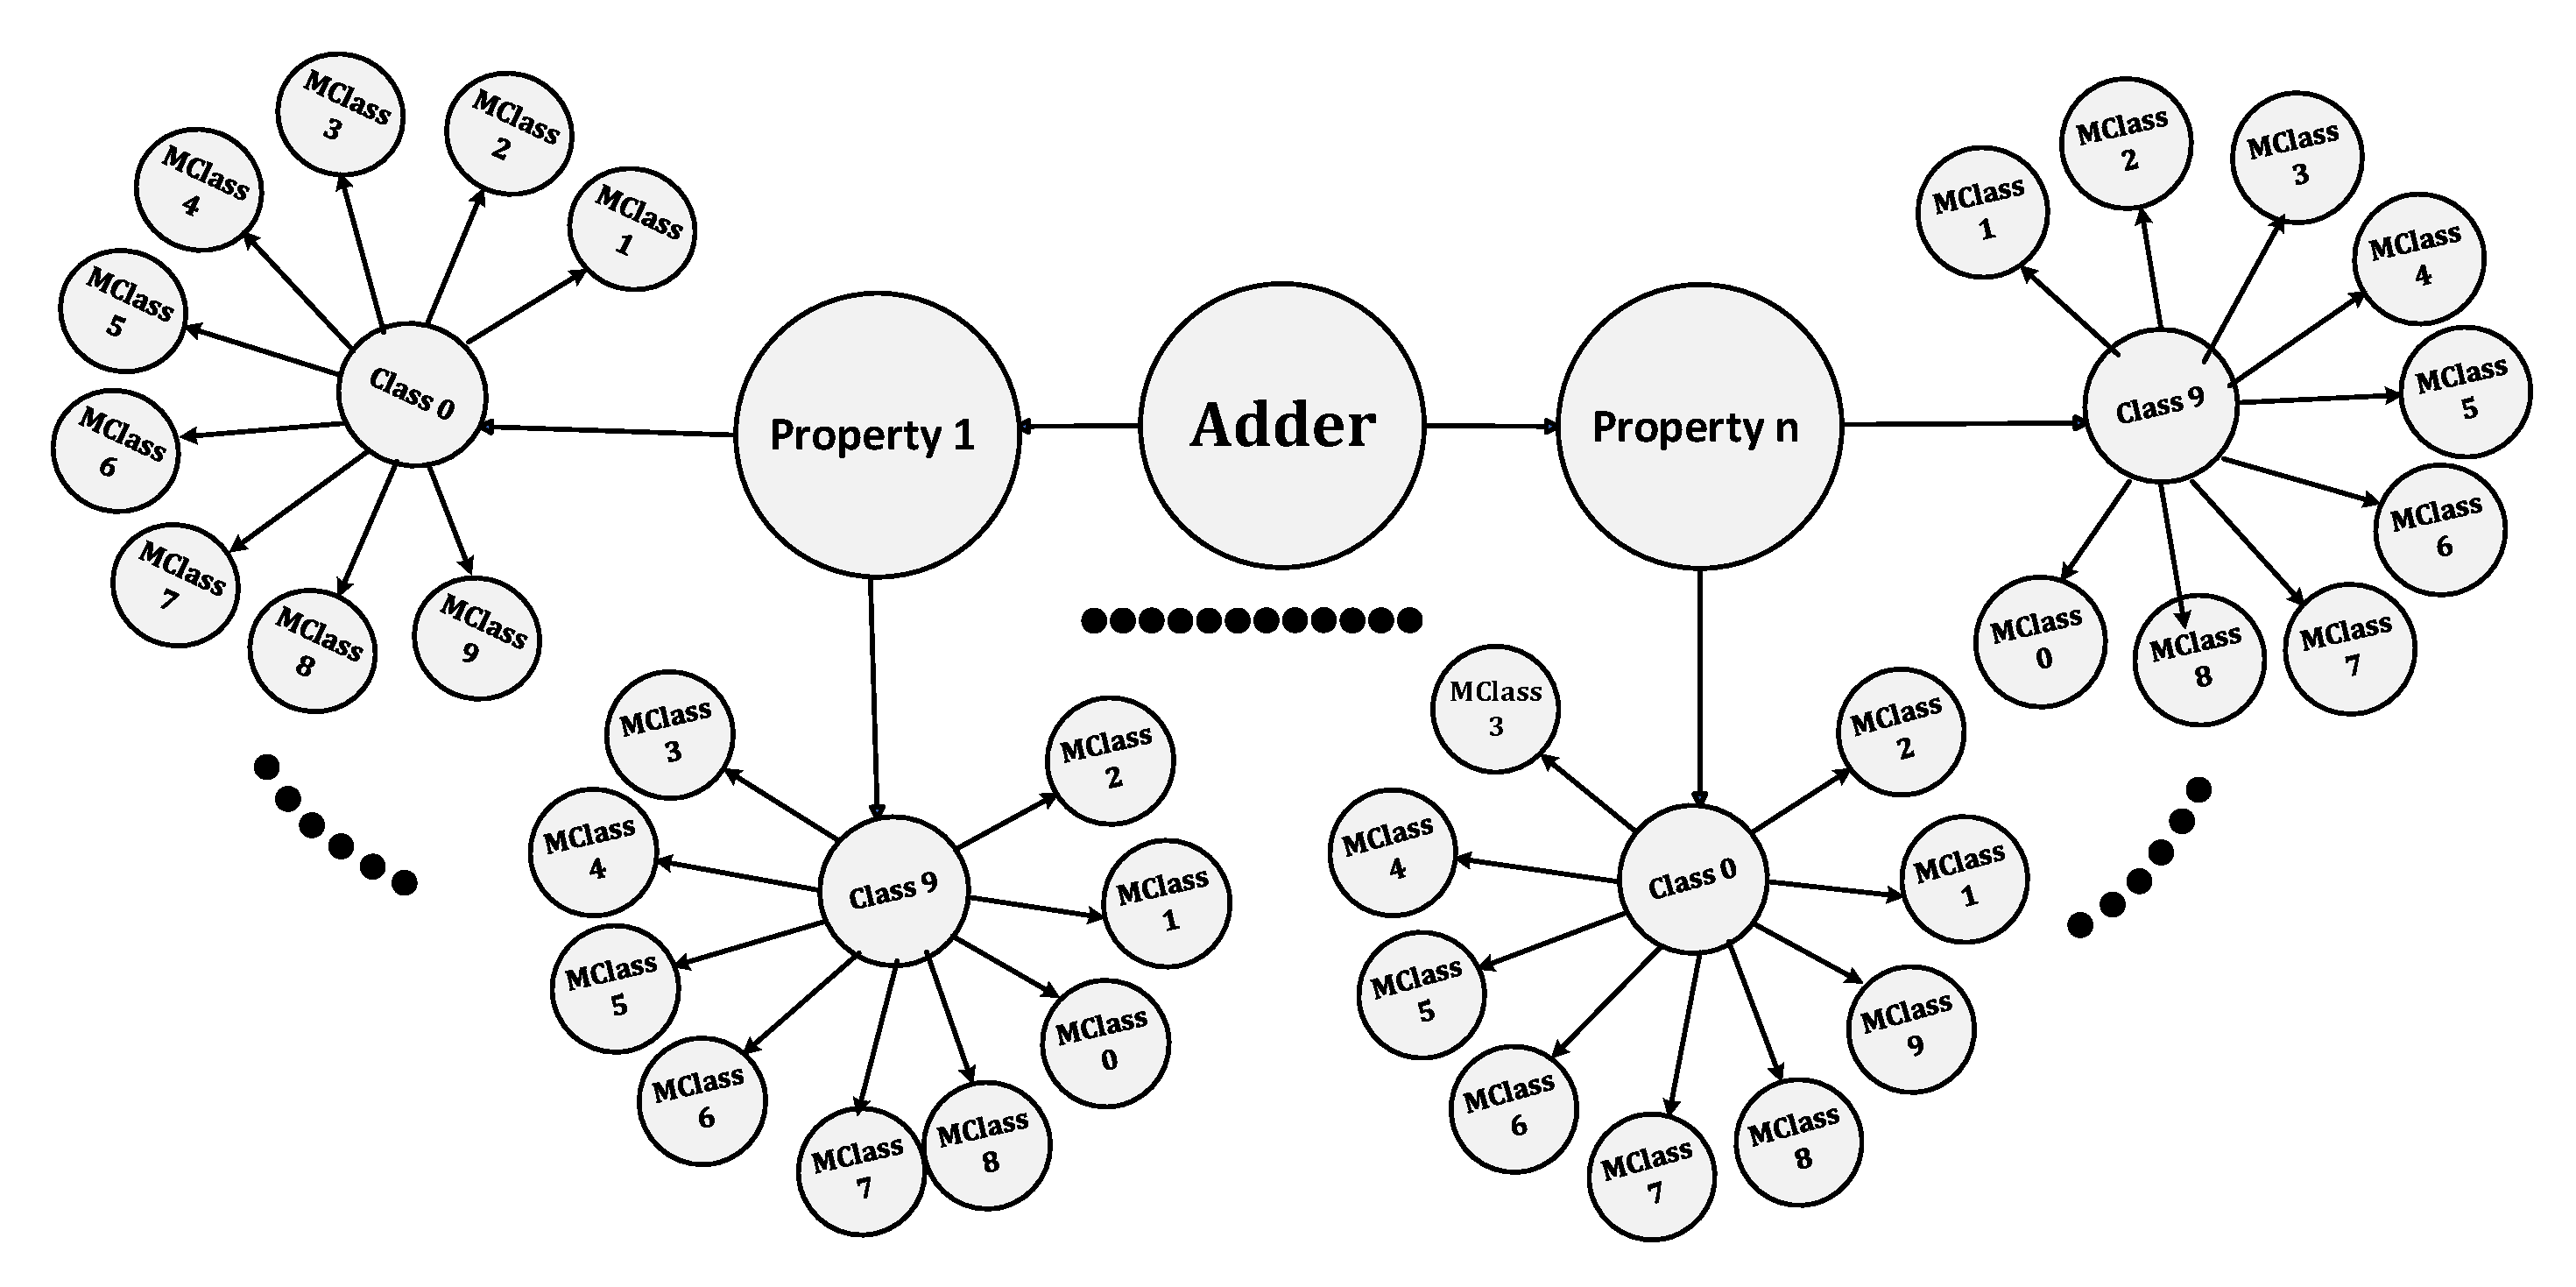
\includegraphics[width=\linewidth]{paper_images/step5.pdf}
    \caption{Diagram of Error Summarization Highlighting Class-Property Impact}
    \label{fig:error-summarization}
\end{figure}

\section{Experiments}

\section{Research Questions}

This paper addresses the following research questions applicable to various vision models and datasets:

\begin{itemize}
    \item How can we design a comprehensive framework to test system correctness?
    \item How can we systematically evaluate the correctness both at local and global levels within framework?
    \item How can error summarization be employed to quantify the impacts on model correctness?
 
\end{itemize}
\section{Threats to Validity}

This section outlines significant limitations and assumptions in our study that may affect the validity and reliability of our findings.

\begin{itemize}
    \item \textbf{Random Sampling:} Our current approach assumes a uniform distribution of samples across all classes, which may not represent the true complexity and variability within real-world data. This uniform sampling can lead to biased evaluations if the class distribution in practical applications is skewed or non-uniform. We plan to enhance our sampling techniques to better capture the diversity and distribution of data in realistic scenarios. Improved sampling strategies will help in developing more robust and generalizable error summarization methods.
\end{itemize}


\section{Conclusion}
% Your conclusion here

\begin{thebibliography}{01}

    \bibitem{dnn_archi}Liu, W., Wang, Z., Liu, X., Zeng, N., Liu, Y. and Alsaadi, F.E., 2017. A survey of deep neural network architectures and their applications. Neurocomputing, 234, pp.11-26.
    \bibitem{Hassija}Hassija, V., Chamola, V., Mahapatra, A., Singal, A., Goel, D., Huang, K., Scardapane, S., Spinelli, I., Mahmud, M. and Hussain, A., 2024. Interpreting black-box models: a review on explainable artificial intelligence. Cognitive Computation, 16(1), pp.45-74.

    \bibitem{Liang}Liang, Y., Li, S., Yan, C., Li, M. and Jiang, C., 2021. Explaining the black-box model: A survey of local interpretation methods for deep neural networks. Neurocomputing, 419, pp.168-182.
    
    \bibitem{adv_attacks}Ren, K., Zheng, T., Qin, Z. and Liu, X., 2020. Adversarial attacks and defenses in deep learning. Engineering, 6(3), pp.346-360.

    \bibitem{deeptest}Tian, Y., Pei, K., Jana, S. and Ray, B., 2018, May. Deeptest: Automated testing of deep-neural-network-driven autonomous cars. In Proceedings of the 40th international conference on software engineering (pp. 303-314).
    
    \bibitem{deepxplore} Pei, K., Cao, Y., Yang, J. and Jana, S., 2017, October. Deepxplore: Automated whitebox testing of deep learning systems. In proceedings of the 26th Symposium on Operating Systems Principles (pp. 1-18).

    \bibitem{deepguage}Ma, L., Juefei-Xu, F., Zhang, F., Sun, J., Xue, M., Li, B., Chen, C., Su, T., Li, L., Liu, Y. and Zhao, J., 2018, September. Deepgauge: Multi-granularity testing criteria for deep learning systems. In Proceedings of the 33rd ACM/IEEE international conference on automated software engineering (pp. 120-131).
    
    \bibitem{SunY}Sun, Y., Huang, X., Kroening, D., Sharp, J., Hill, M. and Ashmore, R., 2018. Testing deep neural networks. arXiv preprint arXiv:1803.04792.

    \bibitem{KimJ}Kim, J., Feldt, R. and Yoo, S., 2019, May. Guiding deep learning system testing using surprise adequacy. In 2019 IEEE/ACM 41st International Conference on Software Engineering (ICSE) (pp. 1039-1049). IEEE.
  
    \bibitem{dlfuzz}Guo, J., Jiang, Y., Zhao, Y., Chen, Q. and Sun, J., 2018, October. Dlfuzz: Differential fuzzing testing of deep learning systems. In Proceedings of the 2018 26th ACM Joint Meeting on European Software Engineering Conference and Symposium on the Foundations of Software Engineering (pp. 739-743).

    \bibitem{tensorfuzz} Odena, A., Olsson, C., Andersen, D. and Goodfellow, I., 2019, May. Tensorfuzz: Debugging neural networks with coverage-guided fuzzing. In International Conference on Machine Learning (pp. 4901-4911). PMLR.

    \bibitem{deepconcolic}Sun, Y., Huang, X., Kroening, D., Sharp, J., Hill, M. and Ashmore, R., 2019, May. DeepConcolic: Testing and debugging deep neural networks. In 2019 IEEE/ACM 41st International Conference on Software Engineering: Companion Proceedings (ICSE-Companion) (pp. 111-114). IEEE.

\end{thebibliography}
\end{document}
